\chapter{Server-Virtualisierung}

\section{Grundlagen}
Überall kann man Virtualisierung einsetzen. Ob bei Server, Speicher, Applikation, Desktops oder Netzwerk. Mit Virtualisierung will man die Abstraktion von der darunterliegende Geräteschaft erreichen.

\subsection{Virtualisierungsarten}
\label{sec:virtualisierungsarten}
\begin{description}
	\item[HW Partitionierung] Teuer, nur noch auf High End Computer anzutreffen. Wie IBM/z, p Systems, Sun/Oracle Sparc.
	\item[HW Virtualisierung] Mittels Hypervisor.
	\item[OS Virtualisierung] Junge, leichtgewichtige Virtualisierungsart. 
\end{description}

\texttt{Partitionierung: Aufteilung eines Dinges in mehrere unabhängige Elemente.}

\subsection{Gründe für eine HW Virtualisierung}
\label{sec:gruende-hw-virtualisierung}
\begin{itemize}
	\item Ressourcen Optimierung
	\item Konsoldierung
	\item Maximierung der Uptime
	\item Schutz der Applikation von Serverausfällen
	\item Einfache Migration wenn Anforderungen wechseln
	\item Schutz der Investitionen in existierende ''legacy Systeme'' 
\end{itemize}

\subsection{Geschichte}
IBM virtualisiert auf den Mainframes bereits in den 60er Jahren. Die Virtualisierung der x86-Systeme wurde erst 1999 eingeführt, durch VMWare. Citrix hat 2007 mit Xen/Xen-Server virtualisiert und Mircosoft im 2008 mit Window Server 2008 und Hyper-V.

\subsection{Was bedeutet Virtualisierung?}
\label{sec:was-bedeutet-virtualisierung}
Darüber streiten sich Joho und die Geister. Was ist Emulation? Simulation? Imitation?  Virtualisation?
\begin{description}
	\item[Emulation] Ein System ahmt ein anderes System nach. Es bekommt den selben Input. Die Verarbeitung wird emuliert. Das führt dazu, dass der Output gleich oder nur fast gleich ist.
	\item[Simulation] Zu Grunde liegt ein Modell, welches die Schlüssel-Charakteristika des zu Simulierenden repräsentiert.
	\item[Virtualität] Eigenschaft einer Sache, nicht in der Form zu existieren, in der sie zu existieren scheint.
	\item[Virtualisierung] Bezieht sich auf den Vorgang der Erstellung einer virtuellen (nicht tatsächlich existenten) Version von etwas. Beispiel: Computer-Hardware, OS, Speichergeräte, Computer-Netzwerk-Ressourcen. 
\end{description}

\subsection{Die drei Anforderungen von Popek und Goldberg}
\label{sec:popek-goldberg-anforderungen}
Diese Anforderungen gelten sowohl ans physische wie auch virtuelle System.
\begin{description}
	\item[Gleichheit] Jedes Programm verhält sich auf beiden Systemen genau gleich. Wichtig!
	\item[Effektivität] Es soll, wann immer möglich, alle Instruktionen direkt auf dem physischen Prozessor ausgeführt werden. Ohne Intervention der VMM.
	\item[Ressourcenkontrolle] VMM hat die komplette Kontrolle über Ressourcen wie Memory, I/O der Peripheriegeräte, aber nicht umbedingt über Prozessoraktivität. Es muss für jedes Programm unmöglich sein die System Ressourcen (wie verfügbares Memory) zu beeinflussen. Der Verteiler (Allocator) muss jedesmal aufgerufen werden.
\end{description}

\subsection{VMM - Virtual Machine Monitor}
\label{sec:vmm-virtual-machine-monitor}
\begin{figure}[h!]
	\centering
	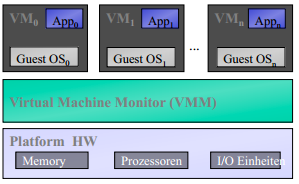
\includegraphics[width=0.4\linewidth]{fig/vmm}
	\caption{VMM}
	\label{fig:vmm}
\end{figure}
Die VM ist die Umgebung erzeugt vom VMM. Die VMM ist eine System Software Schicht und besteht aus folgenden drei Teilen:
\begin{description}
	\item[Dispatcher] dessen Initial Instruction am Speicherplatz liegt wohin die HW trapped.
	\item[Allocator] der entscheidet wer welche Systemressourcen bekommt. Er hat 1 oder n Member (VM).
	\item[Interpreter] für alle Instruktionen die trappen, eine Interpreter Routine pro privilegierte Instruktion.
\end{description}

\subsection{Instruktionsklassifikation}
Es gibt zwei Betriebsmodis.
\begin{itemize}
	\item Uneingeschränkter Supervisor Modus
	\item Eingeschränkter User Modus
\end{itemize}
Eine privilegierte Instruktion verursacht einen Trap im User Modus. Im Supervisor Modus gibt es keinen Trap. Kontrollkritische Instruktionen (control sensitive) versuchen die Config der Systemressourcen zu ändern.

\subsection{Vorteile (Hypervisor) Virtualisierung}
Möglichkeiten, welche die Hypervisor Technologie mitbringt:
\begin{figure}[h!]
\centering
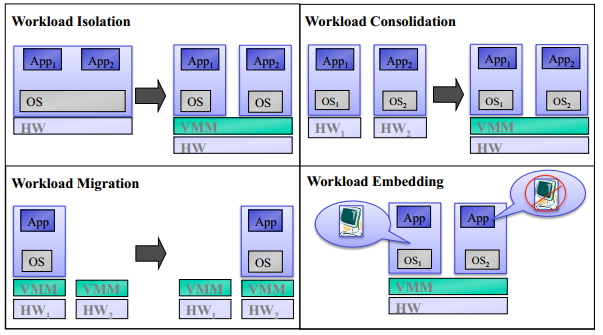
\includegraphics[width=0.7\linewidth]{fig/vorteile-hypervisor-virtualisierung}
\caption{Vorteile Hypervisor Virtualisierung}
\label{fig:vorteile-hypervisor-virtualisierung}
\end{figure}

\subsection{Challenges beim Betrieb einer VMM}
Die Challenges gelten wohl für die VMM und nicht für den Sysadmin, der das System betreibt.
\begin{itemize}
	\item BS und APP wissen nicht, dass eine VMM existiert.
	\item VMM sollte SW Stack gegenüber anderen VMs isolieren.
	\item VMM sollte vor allen anderen Gast-SW geschützt laufen.
	\item VMM sollte eine ''virtuelle Plattform Interface'' zu den Gast-SW präsentieren.
\end{itemize}

\newpage
\section{X86-Virtualisierung}
Poppek und Goldberg sagen, dass eine CPU virtualisierbar ist, wenn alle privilegierten Instruktionen eine Exception erzeugen, wenn sie im unprivilegierten Modus laufen.

\subsection{Theorem 1}
\label{sec:poppek-goldberg-theorem1}
Für beliebige Prozessorarchitekturen der dritten Generation kann
eine effektive VMM aufgebaut werden, wenn der Satz der
kontrollkritischen Instruktionen für eine Prozessorarchitektur
eine Untermenge des Satzes der privilegierten Instruktionen
darstellt.
Im Prinzip besagt das Theorem, das es, um einen VMM zu bauen
genügt, wenn alle Instruktionen, die das korrekte funktionieren
der VMM beeinflussen können (kontrollkritische Instruktionen)
immer (ge)trapped werden und zur Kontrolle an die VMM
weitergegeben und verarbeitet (emuliert) werden.

\subsection{Theorem 2}
Eine beliebige Prozessorarchitekturen der dritten Generation ist
rekursiv virtualisierbar, wenn: Sie selbst virtualisierbar ist und für sie ein VMM ohne Zeitabhängigkeiten konstruiert werden
kann.
Einige Architekturen, wie zum Beispiel die x86-Architektur ohne
hardwaregestütze Virtualierungsfunktionen, erfüllen diese
Bedingungen nicht, weswegen sie nicht auf dem klassischen Weg
virtualisierbar sind.

\subsection{Hypervisor}
Das Problem ist, dass man nicht mehrere BS auf einem physikalischen Rechner laufen lassen kann. Da diese konstruiert sind alle Ressourcen zu managen. Daher braucht es eine Zwischenschicht, welche die BS isoliert. Das BS erfährt somit keine Änderung. Der Hypervisor kommt zum Zug.

\begin{figure}[h!]
\centering
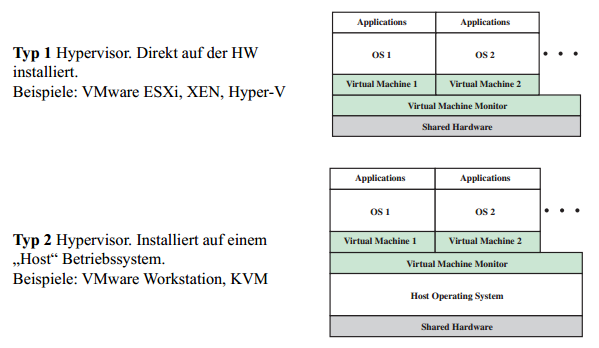
\includegraphics[width=0.8\linewidth]{fig/hypervisor-types}
\caption{Hypervisor Arten}
\label{fig:hypervisor-types}
\end{figure}

\section{HW-Virtualisierung}
\subsection{Direct Exceution}
Es gibt Sicherheitsringe. Die x86 Architektur kennt 4 Ringe. User Level Programme laufen im Ring 3. Das OS brauch HW Zugriff und läuft auf Ring 0. Eine Virtualisierungsschicht muss unter Ring 0 gelegt werden oder es braucht eine Schnittstelle vom Hypervisor mit speziellen Befehlssatz. 
\begin{figure}[h!]
\centering
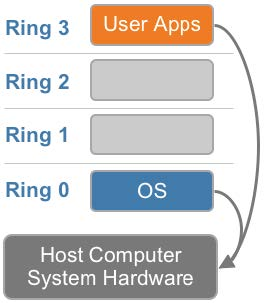
\includegraphics[width=0.4\linewidth]{fig/sicherheitsringe}
\caption{Sicherheitsringe}
\label{fig:sicherheitsringe}
\end{figure}
CPU hat mittels den Sicherheitsringe die Möglichkeiten ob die Instruktionen auch das entsprechende Privileg haben. Der Prozess hat die Möglichkeiten mittels eines Algorithmus zu prüfen ob die Instruktionen von einem privilegierten Memory Segment kommen.

\subsection{Binary Translation}
Im Mainframe wird für jede privilegierte Instruktion ein Trap ausgeführt. Die VMM fängt diese Instruktion ab und emuliert diese. Im x86 ISA sind nicht alle privilegierten Instruktionen Trap geschützt z.B. POPF. Wird diese bswp. im Ring 1 ausgeführt, interessiert das die CPU nicht und wird nicht ausgeführt. Insgesamt gibt es 17 solcher ''nicht abgefanger'' Instruktionen. Abhilfe schafft die binary Translation von VMWare (patentiert!).

Im Bild sieht man, dass es eine Kombination zwischen direkter Ausführung und binary Translation ist. User Level Code wird direkt ausgeführt. Übersetzer Kernel Code ersetzt nicht virtualisierbare Instruktionen. Keine HW Unterstützung nötig. Gast OS voll abstrahiert. User Applikationen laufen direkt und werden nur übersetzt, wenn der GAST-OS Kernel aufgerufen wird.
\begin{figure}[h!]
\centering
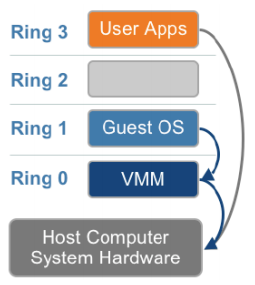
\includegraphics[width=0.4\linewidth]{fig/binary-translation-virt}
\caption{Binary Translation Virtualisation}
\label{fig:binary-translation-virt}
\end{figure}
Ein nativer System Call braucht 242 Prozess Zyklen. Ein Binary translated System Call braucht 2308 Zyklen!

\subsection{Para Virtualisation (SW Assist)}
Para (neben) bezieht sich auf Kommunikation zwischen Gast OS und Hypervisor um die Geschwindigkeit zu erhöhen. Aber der Kenel vom OS muss modifiziert werden um nicht virtualsierbare Instruktionen mit Hypercalls zu ersetzen. Die direkt mit dem Virtualization Layer schwatzen. Hypervisor stellt Hypercall Interface zur Verfügung.
Para ist ziemlich ähnlich wie Binary Translation. Statt im Binary direkt im Source Code! Para braucht keine Laufzeitübersetzung und ist daher schneller. Aber, unveränderte BS können nicht ausgeführt werden! Der grosse Pain.
\begin{figure}[h!]
\centering
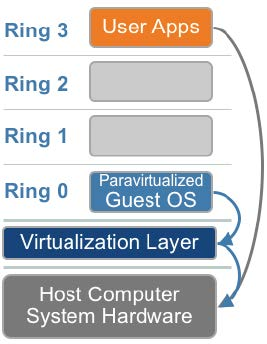
\includegraphics[width=0.4\linewidth]{fig/sw-virtualisierung-ringe}
\caption{Software unterstützte Virtualisierung}
\label{fig:sw-virtualisierung-ringe}
\end{figure}



\subsection{Full Virtualisation (HW Assist)}
\label{sec:hw-unterstuetzt-virt}
VMM und VM haben getrennte Addressbereiche. Dafür musste man neue Operationsmodis kreieren. VMX root (voll privilegiert für VMM) und VMX non-root (nicht voll privilegiert für Gast-VM). Dies reduziert die Gast-VM SW Privilegien ohne auf die Ringe zurückgreifen zu müssen. Dieser neue CPU Modus erlaubt Ringe unterhalb Ring 0. Privlegierte Operatonion gelangen so direkt zum Hypervisor. Der Gast Status wird in virtual machine control structures abgespeichert.
\begin{figure}[h!]
\centering
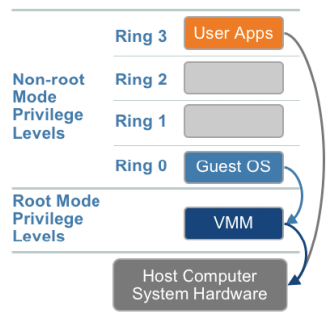
\includegraphics[width=0.4\linewidth]{fig/hw-virtualisierung-ringe}
\caption{Hardware-Virtualisierung Ringe}
\label{fig:hw-virtualisierung-ringe}
\end{figure}

\subsubsection{VMM Lifecycle}
\label{sec:vmm-lifecycle}
\begin{description}
	\item[VM Entry] Übergang VMM zu Gast. Eintritt von VMX non-root Operationen. VMLaunch - Instruktionen werden beim initialen Eintritt verwendet. VMResume - Instruktionen werden beim nachfolgenden Eintritten verwendet.
	\item[VM Exit] Übergang von Gast zu VMM. Eintritt in VMX root Operationen. Speichert Gast Status in VMCS.
\end{description}


\newpage
\section{Memory-Virtualisierung}
Physikalisch mapped das OS virtual Page Number zu physical Page Number. Eine VM denkt, dass es physisches Memory vor sich hat und kann so agieren. Aber dieses Memory wird durch den Hypervisor verwaltet. Das gesamte Memory der Maschine wird durch alle VMs geteilt. Der Dreh- und Angelpunkt ist der Hypervisor.

\subsection{Memory Verbrauch}
\label{sec:ballooning}
Man kann mit folgenden Möglichkeiten Memory sparen, auch bekannt als Memory Rückgewinnungstechnologien:
\begin{description}
	\item[Page Sharing] In homogenen Gast Systemen findet sich viele identische Pages. Algorithmus: Scan all pages, Hash per page, Hash-Collision means same page, check byte by byte, mark as read only. Falls nun doch einer schreiben möchte, wird dies kopiert.
	\item[Page Patching] ''Fast gleiche'' Pages gibt es sehr viele. Bei nur wenig Differenz von Pages werden die als ''fast gleich'' beurteilt. VM 1 arbeitet schlussendlich mit der echten Page. Die VM 2 arbeitet schlussendlich mit der Page von der VM 1 und einer Differenz, welches Teil einer anderen Page ist.
	\item[Page Compression] Es gibt viele Pages die in naher Zukunft nicht verwendet werden. Diese können komprimiert werden.
	
	\item[Ballooning] Vergesst die Papers von Bruno (wirklich!). Es ist simpel. Ballooning erlaubt es dem Hypervisor ungenutztes Memory von den VMs abzuziehen und es anderen VMs zur Verfügung zu stellen. Ein Beispiel: Wir haben mehrere VMs mit 8GB alloziert. Die meisten verwenden jedoch nur 4GB effektiv. Nun braucht eine einzelne aber gerade für einen intensiven Prozess 12GB. Nun kommt die Ballooning Technologie zum Einsatz. Der Hypervisor nimmt von den anderen VMs das nicht gebrauchte Memory und stellt es der VM zur Verfügung, welche es tatsächlich braucht. Da das Gast-BS innerhalb der VM läuft, weiss es nicht wie der Total Amount of Memory des physischen Hosts ist. Ballooning macht dem Gast-BS bewusst, über die Speicherknappheit des Hosts. Achtung: Auf der VM muss ein Balloon-Treiber installiert sein.
\end{description}

\newpage
\section{OS Virtualisierung}
''Hypervisors are the living proof of operating systems's incompetence''. Hypervisor dienen dazu um die Mängel der OS auszugleichen. Nun kommt die OS Virtualisierung, die Antwort der OS Hersteller.
Es werden keine Hypervisor verwendet, also kein ''Trap and Emulate''. Braucht daher auch nur ganz wenige zusätzliche Prozessorzyklen, es wird nur ein Kern verwendet! (Solaris kann auch mit mehreren Kernen arbeiten)

\subsection{Container / Zone}
Eine Instanz eines virtuellen OS wird Container (Linux) oder Zone (Solaris) genannt. Eine virtuelle OS Instanz ohne eingeschalteten Ressourcen Mgmt. ist nicht für die Produktion geeignet.

\subsection{VMs vs. Container}
VMs sind schwergewichtig, Container sind leichtgewichtig. Die Provisionierung (Bereitstellung) einer VM dauert einiges länger als eines Containers!
\begin{figure}[h!]
\centering
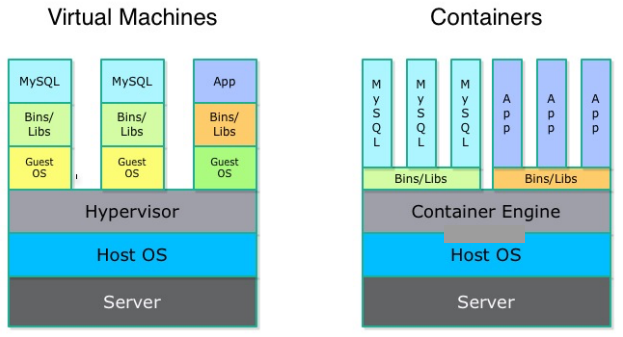
\includegraphics[width=0.7\linewidth]{fig/vms-vs-containers}
\caption{VMs vs. Containers}
\label{fig:vms-vs-containers}
\end{figure}

\subsection{Was kann die OS Virtualisierung?}
\begin{itemize}
	\item Feingranulare Kontrolle der individuellen Prozesse und Applikationen.
	\item Sichere Isolation von Applikationen.
	\item Transparente Migration von Applikationen (siehe Docker) möglich. (Anmerkung: Der Hypervisior migriert nur ganze OS Instanzen.)
\end{itemize}

\subsection{Was kann OS Virtualisierung nicht?}
\begin{itemize}
	\item Keine fremden OS möglich. Auf Windows kann ich nur Windows bringen.
	\item Zonen müssen auf dem selben Patch Level laufen wie OS/Kern.
	\item Anforderungen an SysAdmin steigen.
	\item Ressourcen Mgmt. muss eingeschalten werden (Solaris).
\end{itemize}

\subsection{Container-Architektur}
\begin{figure}[h!]
\centering
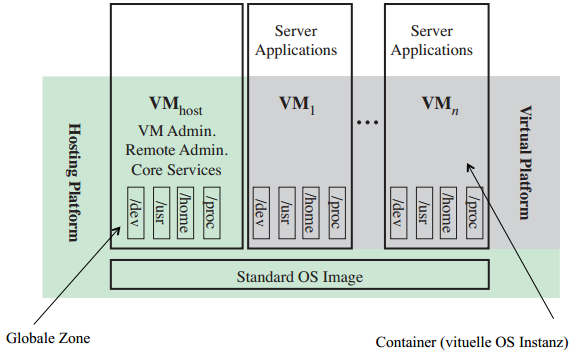
\includegraphics[width=0.7\linewidth]{fig/container-architektur}
\caption{Container-Architektur}
\label{fig:container-architektur}
\end{figure}

\subsection{Beispiel: Linux OS Virtualisierung}
\subsubsection{VServer}
Eine sehr leichtgewichtige Art der OS Virtualisierung. Es benötigt nur eine Instanz des Linux Kernel. VServer benötigt nur ein paar wenige Modifikationen im Kern und ein paar OS Userland Tools. Der Kern verwaltet alle System Ressourcen.

Alle virtuellen OS Instanzen sind isoliert von einander:
\begin{description}
	\item[chroot] - File System Isolation - Damit wird das Root-Directory (/) an einen anderen Ort gelegt. Das modifizierte Umfeld nennt man chroot jail.
	\item[chcontext] - Process Isolation - Ein Linux Utilty, welches einen neuen Security Kontext erzeugt und die Kommandos darin ausführt. Jede OS Instanz verfügt über einen eigenen Prozess-Ausführungskontext.
	\item[chbind] - Network Isolation - Dieses Kommando ist ein System Call. Lockt den resultierend Prozess mit seinen Kinder zu einer spezifischen IP Adresse.
	\item[capablities] - Root User Isolation - Partitioniert die Privilegien eines Root-Users. 
\end{description}

\subsection{Isolation}
Linux Container - Es braucht also drei wichtige Erweiterungen.
\begin{description}
	\item[chroot] Filesystemgrenze für Prozesse -
	\item[cgroups]  - Ressourcen sharing zwischen Prozess Gruppen - Kernel Feature - Erlauben das feingranulare Allozieren von System Ressourcen wie CPU, Memory, Disk über eine Gruppe von Prozessen. CGroups sind hierarchisch gegliedert. Child erbt von Parent. Da alle Prozesse aus der init-Prozess ein Child von einem anderen Prozess ist, nennt man das Mono-Hierarchie (Einzel-Baum).  Beim Erzeugen eines Child-Prozess erbt der Prozess den Umgebungskontext wie die PATH Variabel uvw. vom Parent. Im Unterschied zum herkömmlichen Modell (single-tree), haben wir mit cgroups mehrere unanbhängige Prozess-Bäume. Bsp: memory (setzt limiten auf den Memory Vebrauch), freezer, devices usw.
	\item[ns] - Namespaces - Die Implementation von Container ist eine offensichtliche Verwendung von Namespaces. Ein Namespace abstrahiert eine globale Ressource in der Art, dass der zum Namespace gehörende Prozess meint, ihm gehört die Ressource einzigartig. Änderungen an der globalen Ressourcen sind nur sichtbar für diejenigen, welche im gleichen Namensraum sind. Bsp: PID namespaces isolieren den Prozess ID Namensraum (pro Container unique, aber so mehrere init Prozess mit ID 1 über mehrere Container möglich). Weitere User namespaces, Network, IPC, UTS, Mount namespaces.
\end{description} 

\subsection{Docker}
Wir kennen nun die Linux Container. Mit Docker geht man eine Stufe tiefer. Ein Host hat n-Base Images. Das ist das OS wie Ubuntu, Redhat. Pro Base-Image kann man VMs hinzufügen. Eine VM repräsentiert eine Applikation. Wie PHP, MySQL, Wordpress.

Docker verwendet die Möglichkeit von LXC. Solche Container sind read-only und hoch portierbar. Dies ist ein Software-Layer über dem LCX. Dockt wortwörtlich an jedes Linux an.

\begin{figure}[h!]
\centering
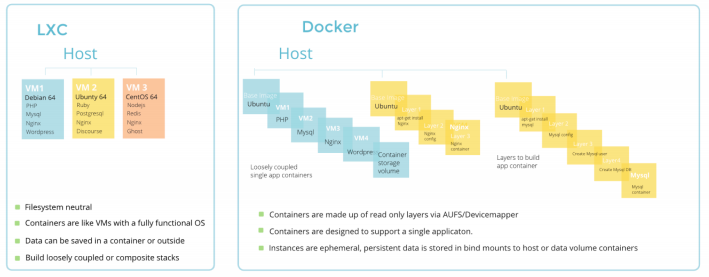
\includegraphics[width=0.9\linewidth]{fig/lxc-vs-docker}
\caption{LXC vs. Docker}
\label{fig:lxc-vs-docker}
\end{figure}


\section{Lernziele}

\section{Fragen}
\subsection{Wann ist eine CPU nach Poppek u. Goldberg virtualisierbar?}
''Nach Popek und Goldberg ist eine CPU (ISA) virtualisierbar, wenn
alle privilegierten Instruktionen eine Exception erzeugen, wenn sie
in einem unprivilegierten Prozessormodus ausgeführt werden.
Alle sensiblen Instruktionen sind privilegiert''

\subsection{Was versteht man unter Emulation?}
Siehe Abschnitt \ref{sec:was-bedeutet-virtualisierung}

\subsection{Erklären Sie nach Poppek u. Goldberg das ''mapping der virtuellen Maschine'' und den darin verwendeten Homomorphismus!}
Siehe Popek und Goldberg Anforderungen 1 \ref{sec:popek-goldberg-anforderungen}

\subsection{Nennen Sie ein paar verschiedene Virtualisierungen die eine wichtige Rolle im Datacenter spielen!}
Siehe Abschnitt \ref{sec:virtualisierungsarten}

\subsection{Nennen Sie die neuen Intel Instruktionen mit denen der (Hypervisor) Programmierer den Eintritt/Austritt in die VM veranlassen kann.}
Siehe Abschnitt \ref{sec:vmm-lifecycle}

\subsection{Was ist eine Virtualisation?}
Siehe Abschnitt \ref{sec:was-bedeutet-virtualisierung}

\subsection{Welche Aufgaben muss eine VMM lösen können?}
Siehe Abschnitt \ref{sec:vmm-virtual-machine-monitor}

\subsection{Wo werden im HW unterstuetzten x86 Sicherheitsmodell der Kern, Hypervisor und die Applikationen ausgefuehrt?}
Siehe Abschnitt \ref{sec:hw-unterstuetzt-virt}. Kern und Hypervisor unter Ring 0, Gast-OS im Ring 0, Applikationen Ring 3.

\subsection{Nennen Sie die Gründe für die HW Virtualisierung!}
Siehe Abschnitt \ref{sec:gruende-hw-virtualisierung}

\subsection{Was ist eine Simulation?}
Siehe Abschnitt \ref{sec:was-bedeutet-virtualisierung}

\subsection{Erklaeren Sie das Theorem 1 nach Poppek u. Goldberg!}
Siehe Abschnitt \ref{sec:poppek-goldberg-theorem1}

\subsection{Erklaeren Sie den Vorgang ''Ballooning''!}
Siehe Abschnitt \ref{sec:ballooning}